%% TOSEM special section: Human-AI Collaboration in Software Engineering.
%% Journal-first / fast-impact track. Submission deadline 1 September 2026.
%% Journal-first extension of: AgenticSE '26 (Workshop on Agentic Software
%% Engineering, San Jose, CA, May 2026). Formatted per acmart-primary-3
%% samples/acmsmall-submission.tex.
\documentclass[acmsmall,review,screen]{acmart}

\usepackage{amsmath}
\usepackage{booktabs}
\usepackage{graphicx}
\usepackage{hyperref}
\usepackage{tikz}
\usepackage{pifont}

\emergencystretch=3em

\setcopyright{acmlicensed}
\acmJournal{TOSEM}
\acmYear{2027}
\acmVolume{0}
\acmNumber{0}
\acmArticle{0}
\acmMonth{8}
\acmDOI{}

\received{1 September 2026}

\title{When Query Rewriting Loses the Documents: An Adaptive Multi-Agent RAG
Architecture for Software Ecosystem Update Monitoring}

% Conference version title, retained for reference:
% \title{An Adaptive Multi-Agent RAG Architecture for Software Ecosystem Update Monitoring}

\author{Shradha Devendra Pujari}
\affiliation{%
  \institution{University of the Pacific}
  \department{Department of Computer Science}
  \city{Stockton}
  \state{CA}
  \country{USA}}
\email{s_pujari@u.pacific.edu}

\author{Solomon Berhe}
\affiliation{%
  \institution{University of the Pacific}
  \department{Department of Computer Science}
  \city{Stockton}
  \state{CA}
  \country{USA}}
\email{sberhe@pacific.edu}

\begin{document}

\begin{abstract}
Software ecosystems produce release notes, security advisories, version control
records, and community discussions, and answering a question about a software
update usually requires combining several of them. Retrieval-Augmented
Generation (RAG) is a natural fit, and a common design pattern decomposes the
pipeline into specialized agents, with a query-rewriting agent normalizing user
terminology to the vocabulary of technical documents.

This paper reports that this pattern contains a failure mode that is invisible
to the metric most likely to be used to evaluate it. We built an adaptive
multi-agent RAG architecture for software update questions --- specialized
agents for query rewriting, retrieval, evaluation, and orchestration, with a
retrieval-level feedback loop and a persistent term-weight memory --- and
measured a 17.2\% retrieval improvement over a single-agent baseline on a
keyword-overlap quality score of our own design. Re-scored with standard
information-retrieval metrics over pooled relevance judgments, the same system
\emph{lost} to the same baseline (nDCG@3 0.145 versus 0.765). The
disagreement was not a metric artifact. Because the rewritten query
\emph{replaced} the user's wording at every retrieval endpoint, 22 of the 23
relevant documents the baseline found were never fetched by the multi-agent
pipeline at all. Three successively stronger rerankers raised mean reciprocal
rank from 0.250 to 0.625 while leaving nDCG@3 near 0.19, because reranking
cannot promote a document that was never retrieved. Searching both the original
and the rewritten phrasing and unioning the pools raises nDCG@3 to 0.973 in one
step.

We draw three conclusions for practitioners building agentic software
engineering tools. First, query rewriting must augment retrieval rather than
substitute for it; the distinction is invisible in aggregate scores and decisive
in the retrieved set. Second, a bespoke retrieval-quality metric can invert the
ordering that standard IR metrics produce, so architectural claims resting on
one are not safe. Third, and least comfortable: with both defects repaired, the
multi-agent pipeline \emph{matches} rather than beats the single-agent baseline
at roughly twice the latency, so decomposition per se is not what produced the
original result. We release the architecture, the evaluation harness, and a
300-question benchmark spanning 24 software ecosystems and five question
categories, mined from live release, advisory, and community sources.
\end{abstract}

\keywords{Multi-Agent Systems, Retrieval-Augmented Generation, Query Rewriting,
Retrieval Evaluation, Software Ecosystem Monitoring, Negative Results,
Self-Improving Agents, RLAIF}

\maketitle

\section{Introduction}

Modern software ecosystems produce a diverse collection of documents, including release notes, security advisories, version control records, and online community discussions. These documents contain information about software updates, vulnerabilities, compatibility issues, and deployment considerations. Answering software update--related questions often requires integrating information from multiple sources.

Software update information is frequently accessed through natural language questions. Developers, system administrators, and users commonly ask colleagues about software updates or seek information through online community platforms. Answering such questions often requires locating relevant documents, reviewing information from multiple sources, and evaluating the consistency of available documents. Systems that generate accurate source-grounded answers can reduce the effort required to retrieve, read, and synthesize information from software ecosystem documents.

Retrieval-Augmented Generation (RAG) systems have emerged as a promising approach for answering such questions by combining document retrieval with large language models to generate answers grounded in external information~\cite{lewis2020rag}. Conventional single-agent RAG systems typically perform query understanding, retrieval, evaluation, and answer generation within a single reasoning process. This can result in vocabulary mismatch between user questions and retrieved documents~\cite{gao2024dmqr}, limited handling of domain-specific terminology, and the absence of feedback mechanisms for correcting retrieval errors \cite{cook2025rag}.

Recent multi-agent RAG systems decompose retrieval and reasoning into multiple specialized agents~\cite{wang2024mainrag, nguyen2025marag}. Most existing evaluations focus on general question-answering benchmarks, whereas software update questions require combining information from heterogeneous software ecosystem documents. In addition, the role of feedback-based adaptation in multi-agent RAG systems for software update question answering has received limited empirical evaluation~\cite{ma2023rafe}.

This paper presents an Adaptive Multi-Agent RAG Architecture for answering software update questions \cite{he2025,joshi2025review}. The architecture consists of specialized agents for query rewriting, retrieval, evaluation, and orchestration connected through a feedback loop \cite{ghosh2025event,adimulam2026,roman2026}.

\subsection{A Result We Did Not Expect}

Our first evaluation followed what is, judging by the literature, common
practice: we defined a retrieval-quality score for the domain --- keyword and
source overlap between the question and the retrieved set --- and compared the
multi-agent architecture against a single-agent baseline on 50 real user
questions. The architecture improved that score by 17.2\% ($t(49)=2.32$,
$p=0.020$), improving in every question category. That is the result reported in
the conference version of this work.

Re-scoring the same pipeline with standard information-retrieval metrics ---
nDCG@$k$, Recall@$k$, and MRR over relevance judgments pooled across systems ---
reversed the ordering. The single-agent baseline reached nDCG@3 of 0.765; the
multi-agent architecture reached 0.145. A 17.2\% advantage on one metric
coexisted with a factor-of-five deficit on another, over the same questions, the
same corpus, and the same retrieved documents.

Metric disagreements of this size usually indicate that one metric is measuring
something other than what it claims. That was true here, but not in the
direction we assumed. Investigating the gap produced this paper's central
finding, which we state plainly because it is the part that transfers to other
systems:

\begin{quote}
\emph{The query-rewriting agent's output replaced the user's wording at every
retrieval endpoint. Of the 23 relevant documents the single-agent baseline
retrieved across the evaluation set, 22 were never fetched by the multi-agent
pipeline at all.}
\end{quote}

The rewritten query was not retrieving the wrong documents from a correct
candidate set --- a ranking problem, which is how we first read the evidence and
how the vocabulary-mismatch framing in the literature invites one to read it.
It was constructing a different, smaller candidate set from which the answer was
largely absent. We confirmed the distinction by fixing ranking first: three
successively stronger rerankers scored against the user's original question
raised MRR monotonically from 0.250 to 0.500 to 0.625, while nDCG@3 stayed near
0.19. A ranking fix that cannot close a ranking gap is evidence that the
documents are not there to be ranked. Searching both the original and the
rewritten phrasing and unioning the candidate pools moves nDCG@3 from 0.188 to
0.973 in a single change.

\subsection{Contributions}

\begin{itemize}
  \item \textbf{A failure mode in agentic query rewriting, measured and
  localized.} Rewriting that substitutes for the user's query rather than
  extending it loses relevant documents at the retrieval step. We quantify the
  loss by counting documents rather than inferring it from scores, show that it
  is not recoverable by reranking, and give a remedy that costs one additional
  set of retrieval calls (Sections~\ref{sec:results} and~\ref{sec:discussion}).

  \item \textbf{Evidence that a domain-specific retrieval metric can invert the
  conclusion.} The same architecture, questions, and documents yield opposite
  orderings under our keyword-overlap score and under pooled-judgment IR
  metrics. We report both, with the pooling protocol and judge configuration, as
  a caution for agentic-system evaluations that define their own quality scores.

  \item \textbf{An honest accounting of what multi-agent decomposition bought.}
  With both defects repaired, the multi-agent pipeline reaches parity with the
  single-agent baseline at approximately twice the latency. We report this
  rather than the improvement the original metric showed, and discuss what would
  constitute evidence for decomposition in this domain.

  \item \textbf{An architecture and adaptation mechanism for software ecosystem
  monitoring.} Vendor-aware retrieval across release notes, security advisories,
  and community discussions, a deterministic evaluator agent that triggers
  retrieval retries, and a persistent term-weight memory that adapts retrieval
  behavior without human feedback or model retraining (Section~\ref{sec:method}).

  \item \textbf{A reusable benchmark and harness.} 300 questions spanning 24
  software ecosystems and five question categories, mined from live release,
  advisory, and community sources, with the upstream data defects we found
  documented and handled; plus an evaluation harness computing IR metrics,
  CRAG-style correctness labels, and paired statistics, released with the
  ablation arms that produced every number in this paper.
\end{itemize}

\subsection{Paper Organization}

Section~\ref{sec:related} reviews related work on RAG, multi-agent
decomposition, corrective retrieval, and query rewriting.
Section~\ref{sec:method} describes the architecture and the data sources.
Section~\ref{sec:results} presents the evaluation: the metric disagreement, the
localization of its cause, the ranking ablation, and the effect of the remedy.
Section~\ref{sec:discussion} discusses what generalizes, the limitations we are
able to bound, and the threats we cannot.
Section~\ref{sec:conclusion} concludes.

\section{Related Work}\label{sec:related}

This section reviews prior work on Retrieval-Augmented Generation (RAG),
multi-agent architectures, corrective retrieval, and self-improving
agents. The proposed architecture builds on concepts from each of these
areas.

\subsection{Retrieval-Augmented Generation}

Retrieval-Augmented Generation (RAG) combines document retrieval with
large language models to generate answers grounded in external
documents~\cite{lewis2020rag}. Several extensions have addressed
limitations of fixed retrieval pipelines. DMQR-RAG uses query rewriting
to reduce vocabulary mismatch~\cite{gao2024dmqr}. RaFe introduces
feedback-based reranking of retrieved documents~\cite{ma2023rafe}.
Self-RAG incorporates self-evaluation during generation~\cite{asai2024selfrag},
while Adaptive-RAG selects retrieval logic based on query
characteristics~\cite{jeong2024adaptiverag}. Surveys identify adaptive
retrieval and agent-based coordination as active research directions in
RAG systems~\cite{gao2023survey}.

\subsection{Multi-Agent RAG Frameworks}

Multi-agent RAG systems distribute retrieval and reasoning across
specialized agents. MA-RAG employs planner, extraction, and question
answering agents~\cite{nguyen2025marag}. MAIN-RAG separates document
selection and answer generation through dedicated predictor and judge
agents~\cite{wang2024mainrag}. More generally, frameworks such as
AutoGen~\cite{wu2023autogen} and smolagents~\cite{huggingface2024agents}
provide infrastructure for agent orchestration and tool use. Most prior
evaluations focus on general question-answering benchmarks, whereas this
work evaluates a multi-agent architecture for software update question
answering.

\subsection{Corrective Retrieval and Adaptive Feedback}

Corrective retrieval methods modify retrieval behavior when retrieved
information is insufficient. CRAG evaluates retrieval quality and
initiates additional retrieval when needed~\cite{yan2024crag}. FLARE
performs retrieval conditioned on uncertainty during answer
generation~\cite{jiang2023flare}. Reflexion uses iterative self-feedback
to guide future behavior~\cite{shinn2023reflexion}. The architecture
presented in this paper adopts a similar feedback-oriented perspective
through a dedicated evaluator agent that can trigger retrieval retries
when retrieval quality falls below a predefined threshold.

\subsection{Self-Improving Agents}

RLAIF replaces human preference annotations with AI-generated feedback
signals for system improvement~\cite{bai2022constitutional}. Related
work has explored feedback-driven adaptation in retrieval and generation
systems. Unlike approaches that update model weights, the architecture
proposed in this paper maintains a persistent memory of retrieval
outcomes and uses those outcomes to adjust future query rewriting
without human feedback or model retraining.

\section{Method}\label{sec:method}

This section describes the proposed adaptive multi-agent RAG
architecture for software update question answering. The architecture
decomposes query rewriting, retrieval, evaluation, and orchestration
into specialized agents connected through an adaptive feedback loop. We
also describe the software ecosystem data sources, answer synthesis
process, and experimental setup used in the evaluation.

\subsection{Architecture Overview}

The proposed architecture separates software update question answering
into four specialized agents coordinated by a central Orchestrator.
Rather than performing query understanding, retrieval, evaluation, and
answer generation within a single reasoning process, each task is
assigned to a dedicated component with a defined responsibility. The
architecture consists of a Query Rewriter, Retriever, Evaluator, and
Orchestrator connected through a retrieval-level feedback loop, as
shown in Figure~\ref{fig:architecture}.

The design follows five principles. First, each agent performs a
single task. Second, retrieval is restricted to vendor-specific
information when a vendor can be identified. Third, retrieval quality
is evaluated through an explicit feedback mechanism that can trigger
additional retrieval attempts. Fourth, failures are isolated through
defined input and output contracts. Finally, retrieval outcomes are
persisted across sessions to support adaptation without human
feedback.

\begin{figure}[h]
\centering
\resizebox{\columnwidth}{!}{%
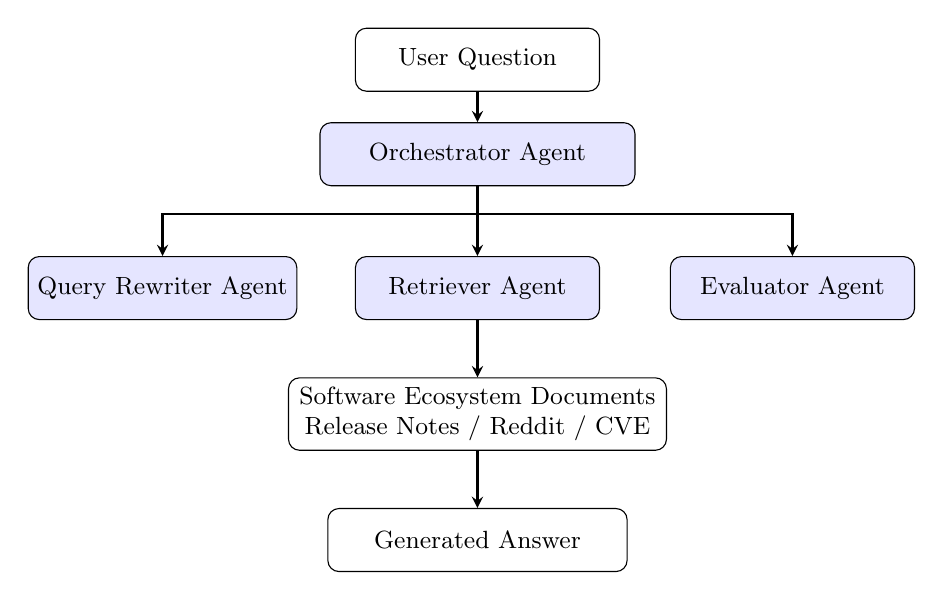
\begin{tikzpicture}[
  box/.style={
      rectangle,
      draw,
      rounded corners,
      text centered,
      align=center,
      minimum height=0.8cm,
      minimum width=3.1cm,
      font=\small,
      fill=white
  },
  agent/.style={
      box,
      fill=blue!10
  },
  arrow/.style={
      ->,
      thick,
      >=stealth
  }
]

% ==================================================
% User Query
% ==================================================

\node[box] (user) at (0,5.2)
      {User Question};

% ==================================================
% Orchestrator
% ==================================================

\node[agent,
      minimum width=4.0cm]
      (orch) at (0,4.0)
      {Orchestrator Agent};

% ==================================================
% Specialized Agents
% ==================================================

\node[agent]
      (rw) at (-4.0,2.3)
      {Query Rewriter Agent};

\node[agent]
      (ret) at (0,2.3)
      {Retriever Agent};

\node[agent]
      (eval) at (4.0,2.3)
      {Evaluator Agent};

% ==================================================
% Documents
% ==================================================

\node[box,
      minimum width=4.8cm]
      (docs) at (0,0.7)
      {Software Ecosystem Documents\\
       Release Notes / Reddit / CVE};

% ==================================================
% Answer
% ==================================================

\node[box,
      minimum width=3.8cm]
      (ans) at (0,-0.9)
      {Generated Answer};

% ==================================================
% Main Flow
% ==================================================

\draw[arrow]
      (user.south)
      -- (orch.north);

\draw[arrow]
      (orch.south)
      -- ++(0,-0.35)
      -| (rw.north);

\draw[arrow]
      (orch.south)
      -- (ret.north);

\draw[arrow]
      (orch.south)
      -- ++(0,-0.35)
      -| (eval.north);

\draw[arrow]
      (ret.south)
      -- (docs.north);

\draw[arrow]
      (docs.south)
      -- (ans.north);

\end{tikzpicture}%
}
\caption{Adaptive multi-agent RAG architecture.}
\label{fig:architecture}
\end{figure}

\subsection{Agent Definitions}

The architecture comprises four agents organized under Orchestrator
coordination.

\textbf{Orchestrator Agent.}
The Orchestrator coordinates execution of the retrieval pipeline. It
receives the user question, delegates tasks to the remaining agents, and
manages retrieval retries when requested by the Evaluator. The
Orchestrator does not perform retrieval or answer generation directly.

\textbf{Query Rewriter Agent.}
The Query Rewriter addresses differences between user vocabulary and
document vocabulary. Llama~3.1~8B is used to transform the original
question into a retrieval-oriented representation. In the self-improving
configuration, learned terms from previous retrieval outcomes are
incorporated before query generation.

\textbf{Retriever Agent.}
The Retriever performs vendor-aware document retrieval. It first
attempts to identify the software vendor referenced in the query using
exact matching, alias lookup, and fuzzy matching against a registry of
14,223 software vendors and 628 software-related subreddits. If a
vendor is detected, retrieval is restricted to vendor-specific
release notes, advisories, and community discussions. Otherwise, a
general retrieval logic is used. The Retriever returns ranked
documents without evaluating their quality \cite{guan2025, zheng2026, yang2026}.

\textbf{Evaluator Agent.}
The Evaluator estimates retrieval quality using a deterministic score
between 0.0 and 1.0. The score combines evidence from retrieval
volume, release-note matches, community matches, and CVE matches. If
the score falls below a predefined threshold ($\theta = 0.30$), the
Evaluator signals the Orchestrator to perform an additional retrieval
attempt. The Evaluator does not generate answers \cite{zhuge2024}.

\subsection{Adaptive Feedback and Self-Improvement}

The architecture incorporates a retrieval-level feedback loop. After
retrieval, the Evaluator assigns a quality score to the retrieved
documents. If retrieval quality is insufficient, the Orchestrator
re-executes the retrieval pipeline using a revised question generated by
the Query Rewriter.

The system also maintains a persistent Self-Improvement Memory. Query
expansion terms accumulate positive or negative scores based on
retrieval outcomes across sessions. Successful retrievals increase
associated term weights, while unsuccessful retrievals decrease them.
These scores are subsequently used by the Query Rewriter to influence
future retrieval queries. This mechanism provides adaptation without
human preference labels, manual annotation, or model retraining.

\subsection{Software Ecosystem Data Sources}

The system retrieves information from software ecosystem documents
obtained through multiple API endpoints.

\textbf{Verified Sources}
\begin{itemize}
\item \texttt{/\{vendor\}}: vendor registry (6,578 entries)
\item \texttt{/v/}: software release notes (31,958 entries)
\item \texttt{/cve}: vulnerability advisories (24,139 entries)
\end{itemize}

\textbf{Community Sources}
\begin{itemize}
\item \texttt{/reddit}: community discussions (208,466 posts)
\item \texttt{/positive}: software update risk discussions (2,637 posts)
\item \texttt{/by-subreddit?q=\{vendor\}}: vendor-specific discussions
\item \texttt{/questions}: software-related user questions
\end{itemize}

To support vendor-aware retrieval, a registry of software vendors and
associated subreddits is loaded at startup and cached locally.

\subsection{Answer Generation}

Retrieved documents are synthesized into a final answer using a
structured prompt. The prompt constrains generation to information
contained in retrieved sources and defines explicit behavior for
common retrieval outcomes.

The synthesis process follows six rules:

\begin{enumerate}
\item Summarize matching community discussions and associated comments.
\item Report version-specific information when present in release notes.
\item Explicitly state when retrieved sources do not directly answer the question.
\item Do not generate unsupported version numbers, fixes, or CVE identifiers.
\item Restrict claims to information contained in retrieved sources.
\item Report when no matching vendor-specific information is available.
\end{enumerate}

\subsection{Experimental Setup}

The evaluation dataset consists of 50 software update questions
spanning security, bug, release, community, and general software
maintenance topics. The local fallback dataset contains 324 Reddit
posts collected through the software ecosystem data lake and filtered
using minimum quality criteria of at least 10 comments, 3 author
replies, and a quality score of at least 0.30.

The single-agent baseline performs query rewriting, retrieval
evaluation, and answer generation within a single agent without
specialized agents, adaptive retry, or self-improvement memory. It
uses the same retrieval endpoints and answer synthesis prompt as the
proposed architecture, isolating the effect of architectural
decomposition.

All experiments were performed using Llama~3.1~8B executed through
Ollama with temperature set to zero. The evaluation platform consisted
of Apple Silicon hardware with 24\,GB memory and Metal GPU
acceleration.

\section{Results}\label{sec:results}

This section presents the evaluation results of the proposed adaptive
multi-agent RAG architecture. The evaluation examines retrieval quality,
answer accuracy, adaptive feedback behavior, self-improvement
performance, representative examples, failure modes, and implementation
observations using a dataset of 50 software update questions.

\subsection{Retrieval Quality}

Table~\ref{tab:quality} summarizes retrieval quality across five
question categories. The proposed architecture achieved higher mean
retrieval quality than the single-agent baseline in all categories. The
overall retrieval quality increased from 0.680 to 0.798, corresponding
to a 17.2\% improvement. A paired $t$-test across the 50 evaluation
queries yielded $t(49)=2.32$ and $p=0.020$.

\begin{table}[h!]
\centering
\caption{Retrieval Quality by Question Category}
\label{tab:quality}
\resizebox{\columnwidth}{!}{%
\begin{tabular}{llccc}
\toprule
\textbf{Rank} & \textbf{Category} & \textbf{1-Agent} & \textbf{4-Agents} & \textbf{Improvement} \\
\midrule
1 & Security & 0.630 & 0.750 & +19.0\% \\
2 & Bugs & 0.756 & 0.833 & +10.3\% \\
3 & Releases & 0.667 & 0.723 & +8.5\% \\
4 & Community & 0.730 & 0.850 & +16.4\% \\
5 & General & 0.600 & 0.750 & +25.0\% \\
\midrule
 & \textbf{Overall} & \textbf{0.680} & \textbf{0.798} & \textbf{+17.2\%} \\
\bottomrule
\end{tabular}
}
\end{table}

Table~\ref{tab:ablation} reports the effect of removing individual
components from the architecture. Vendor-aware retrieval, multi-source
retrieval, and CVE integration each reduced retrieval quality when
removed. The largest reduction was observed when multi-source retrieval
was disabled.

\begin{table}[h]
\centering
\caption{Ablation Study}
\label{tab:ablation}
\resizebox{\columnwidth}{!}{%
\begin{tabular}{llcl}
\toprule
\textbf{Rank} & \textbf{Configuration} & \textbf{Mean Quality} & \textbf{Contribution} \\
\midrule
1 & Our System (all 4 agents) & 0.340 & --- \\
2 & \quad -- Vendor Extraction (fallback only) & 0.325 & +0.015 \\
3 & \quad -- Multi-Source Validation (single tier) & 0.320 & +0.020 \\
4 & \quad -- CVE Integration (releases+Reddit) & 0.321 & +0.019 \\
\bottomrule
\end{tabular}
}
\end{table}

\subsection{Answer Accuracy}

To evaluate answer quality beyond retrieval metrics, the system was
tested on version-specific software update questions. For example, the
system correctly identified Linux v7.0.0 (released April 13, 2026) and
Firefox v149.0.1 (released April 7, 2026) from the corresponding
release sources. All reported version numbers were traceable to
retrieved documents.

A supplementary evaluation using ten questions from the live questions
endpoint produced four fully correct answers and six partially correct
answers. Across these questions, the system did not generate any
unsupported version numbers, release dates, or software update claims.
All version-specific information appearing in generated answers could be
traced to retrieved release notes or other retrieved documents.

Figure~\ref{fig:siri_example} presents a representative software update
question. The question concerns Siri behavior following the iOS~26.4
update. The Retriever identified the relevant vendor, collected
release and community information, and the generated answer reflected
information contained in the retrieved sources.

\begin{figure*}[t]
\centering
\resizebox{\textwidth}{!}{%
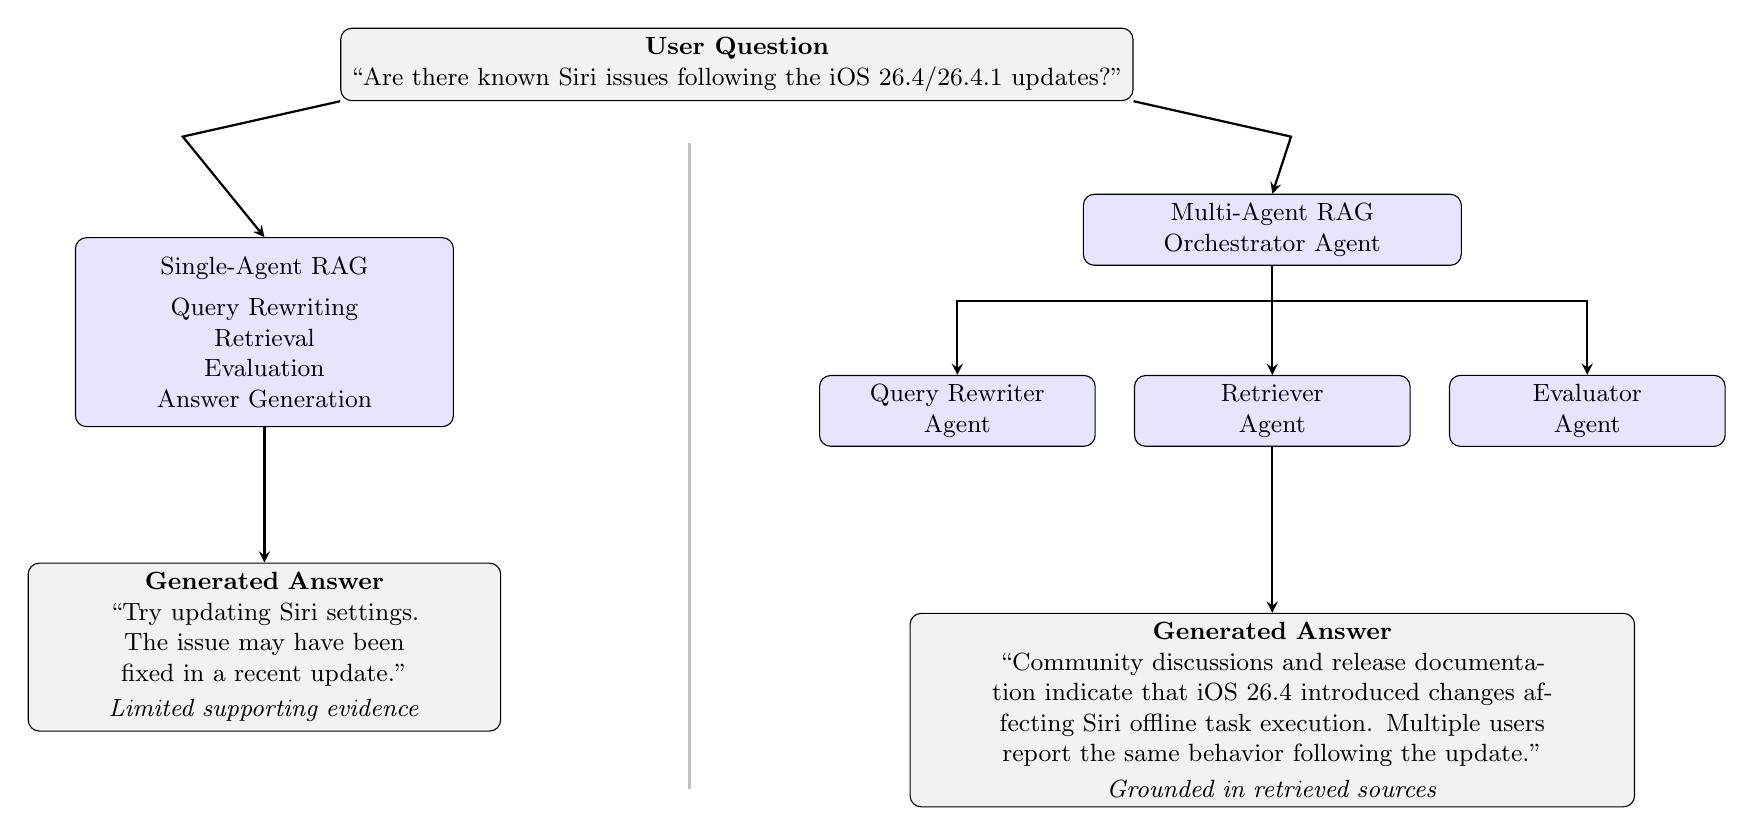
\begin{tikzpicture}[
  box/.style={
      rectangle,
      draw,
      rounded corners,
      text centered,
      align=center,
      minimum height=0.8cm,
      font=\small,
      fill=white
  },
  agent/.style={
      box,
      fill=blue!10
  },
  answer/.style={
      box,
      fill=gray!10
  },
  arrow/.style={
      ->,
      thick,
      >=stealth
  }
]

% ==================================================
% Example Query
% ==================================================

\node[
    box,
    fill=gray!10,
    minimum width=8.2cm
] (query) at (0,6.2)
{
\textbf{User Question}\\
``Are there known Siri issues following the iOS 26.4/26.4.1 updates?''
};

% ==================================================
% Left Side : Single-Agent RAG
% ==================================================

\node[
    agent,
    minimum width=4.8cm,
    minimum height=2.4cm
] (single) at (-6.0,2.8)
{
Single-Agent RAG\\[4pt]
Query Rewriting\\
Retrieval\\
Evaluation\\
Answer Generation
};

\node[
    answer,
    minimum width=6.0cm,
    text width=5.4cm
] (ans1) at (-6.0,-1.2)
{
\textbf{Generated Answer}\\
``Try updating Siri settings. The issue may
have been fixed in a recent update.''\\[2pt]
\textit{Limited supporting evidence}
};

% ==================================================
% Divider
% ==================================================

\draw[gray!50, very thick]
(-0.6,-3.0) -- (-0.6,5.2);

% ==================================================
% Right Side : Multi-Agent RAG
% ==================================================

\node[
    agent,
    minimum width=4.8cm
] (orch) at (6.8,4.1)
{
Multi-Agent RAG\\
Orchestrator Agent
};

\node[
    agent,
    minimum width=3.5cm
] (rw) at (2.8,1.8)
{
Query Rewriter\\
Agent
};

\node[
    agent,
    minimum width=3.5cm
] (ret) at (6.8,1.8)
{
Retriever\\
Agent
};

\node[
    agent,
    minimum width=3.5cm
] (eval) at (10.8,1.8)
{
Evaluator\\
Agent
};

\node[
    answer,
    minimum width=9.2cm,
    text width=8.5cm
] (ans2) at (6.8,-2.0)
{
\textbf{Generated Answer}\\
``Community discussions and release
documentation indicate that iOS~26.4
introduced changes affecting Siri offline
task execution. Multiple users report the
same behavior following the update.''\\[2pt]
\textit{Grounded in retrieved sources}
};

% ==================================================
% Connections
% ==================================================

\draw[arrow]
(query.south west)
-- ++(-2.0,-0.45)
-- (single.north);

\draw[arrow]
(single.south)
-- (ans1.north);

\draw[arrow]
(query.south east)
-- ++(2.0,-0.45)
-- (orch.north);

\draw[arrow]
(orch.south)
-- ++(0,-0.45)
-| (rw.north);

\draw[arrow]
(orch.south)
-- (ret.north);

\draw[arrow]
(orch.south)
-- ++(0,-0.45)
-| (eval.north);

\draw[arrow]
(ret.south)
-- (ans2.north);

\end{tikzpicture}%
}
\caption{
Illustrative comparison of single-agent and multi-agent RAG
architectures on a software update question.
}
\label{fig:siri_example}
\end{figure*}

\subsection{Example Multi-Agent Execution}

Figure~\ref{fig:execution_trace} illustrates a representative execution
of the proposed architecture on a software update question. The Query
Rewriter Agent reformulates the user question to improve retrieval
coverage, the Retriever Agent gathers evidence from software ecosystem
documents, and the Evaluator Agent assigns a retrieval quality score
before answer generation. This example demonstrates how retrieval and
evaluation are separated into specialized agents within the proposed
architecture.

\begin{figure}[t]
\centering
\includegraphics[width=\columnwidth]{Figures/execution_trace.png}
\caption{
Example execution trace of the Query Rewriter, Retriever, and Evaluator agents.
}
\label{fig:execution_trace}
\end{figure}
\subsection{Adaptive Feedback}

The Evaluator triggered retrieval retries when the initial retrieval
quality score fell below $\theta = 0.30$. In these cases, the
Orchestrator executed an additional retrieval cycle using a revised
query generated by the Query Rewriter. This behavior occurred without
manual intervention during evaluation and allowed retrieval to continue
when the initial result set was insufficient.

\subsection{Self-Improvement Behavior}

Retrieval quality increased from a mean score of 0.756 in the first
evaluation tertile ($Q_1$--$Q_{17}$) to 0.826 in the final tertile
($Q_{34}$--$Q_{50}$), corresponding to a 9.3\% increase.

A paired $t$-test comparing the first and last tertiles yielded
$t(16)=2.18$ and $p=0.043$ (two-tailed). The corresponding effect size
was Cohen's $d=0.83$ \cite{cohen1960coefficient}.

During evaluation, 27 query-expansion terms accumulated positive scores
in the Self-Improvement Memory. Table~\ref{tab:learned_terms} lists the
ten highest-scoring terms.

\begin{table}[h]
\centering
\caption{Highest-Scoring Learned Terms}
\label{tab:learned_terms}
\resizebox{\columnwidth}{!}{%
\begin{tabular}{llcl}
\toprule
\textbf{Rank} & \textbf{Term} & \textbf{Cumulative Score} & \textbf{Interpretation} \\
\midrule
1 & vulnerability & +2.20 & Security terminology \\
2 & patch & +1.58 & Fix-related terminology \\
3 & advisory & +1.23 & Advisory terminology \\
4 & update & +1.15 & General update terminology \\
5 & kernel & +0.98 & Vendor-specific terminology \\
6 & release & +0.87 & Version-related terminology \\
7 & bug & +0.76 & Defect-related terminology \\
8 & fix & +0.71 & Resolution terminology \\
9 & version & +0.68 & Version-related terminology \\
10 & security & +0.64 & Security terminology \\
\bottomrule
\end{tabular}
}
\end{table}

\subsection{Representative User Questions and Answers}

Table~\ref{tab:examples} presents representative examples from the
evaluation dataset. The examples include correctly answered queries,
partially relevant answers, and incorrect answers.

\begin{table*}[t]
\centering\small
\caption{Representative Questions Examples}
\label{tab:examples}
\setlength{\tabcolsep}{3pt}
\renewcommand{\arraystretch}{1.1}
\resizebox{\textwidth}{!}{%
\begin{tabular}{p{3.8cm}p{1.45cm}p{4.4cm}p{2.7cm}p{0.7cm}}
\toprule
\textbf{Question} & \textbf{Vendor} & \textbf{Multi-Agent Answer} & \textbf{Evaluator Note} & \textbf{Result} \\
\midrule
\multicolumn{5}{l}{\textit{(A) Correctly Answered}} \\
\midrule
Q1: What is the latest version of Firefox?
   & firefox
   & v149.0.1, released April~7~2026.
   & Exact release note match.
   & \textcolor{green!60!black}{\textbf{\ding{51}}} \\

Q2: Are there known Siri issues following the iOS 26.4/26.4.1 updates?
   & ios
   & iOS~26.4 changed Siri offline mode. r/applehelp confirms.
   & Multiple sources retrieved.
   & \textcolor{green!60!black}{\textbf{\ding{51}}} \\

Q3: G6 Bullet unstable?
   & Ubiquiti
   & Community reports instability; firmware update available.
   & Alias resolved to vendor.
   & \textcolor{green!60!black}{\textbf{\ding{51}}} \\
\midrule
\multicolumn{5}{l}{\textit{(B) Partially Relevant}} \\
\midrule
Q4: Would an IKEA hub update devices more reliably?
   & homeassistant
   & Home Assistant integration information retrieved.
   & Sub-vendor not represented in registry.
   & \textcolor{orange!80!black}{\textbf{$\sim$}} \\

Q5: Can't upload photos on iOS to Immich
   & ios
   & iOS information retrieved; limited Immich coverage.
   & Third-party application not present in vendor sources.
   & \textcolor{orange!80!black}{\textbf{$\sim$}} \\

Q6: Do I have to say goodbye to Windows to switch to Linux?
   & linux
   & General Linux information retrieved.
   & Opinion-oriented question.
   & \textcolor{orange!80!black}{\textbf{$\sim$}} \\
\midrule
\multicolumn{5}{l}{\textit{(C) Incorrectly Answered}} \\
\midrule
Q7: What was the Linux version on January~1st~2026?
   & linux
   & Returned v7.0.0 instead of v6.18.0.
   & Date constraint not applied.
   & \textcolor{red!70!black}{\textbf{\ding{55}}} \\

Q8: Synology NAS unreachable after upgrade
   & (none)
   & No vendor detected.
   & Vendor extraction failure.
   & \textcolor{red!70!black}{\textbf{\ding{55}}} \\

Q9: What small IT task always turns into a nightmare?
   & (none)
   & No relevant documents retrieved.
   & Non-factual question.
   & \textcolor{red!70!black}{\textbf{\ding{55}}} \\
\bottomrule
\end{tabular}
}
\end{table*}

\subsection{Failure Analysis}

The three incorrect examples in Table~\ref{tab:examples} correspond to
three recurring failure modes observed during evaluation.

\paragraph{Temporal Question Filtering.}
The question ``What was the Linux version on January 1st 2026?'' returned
the latest Linux release rather than the release available on the
specified date. The query rewriter preserved the temporal constraint,
but the constraint was not passed to the retrieval endpoint.

\paragraph{Vendor Extraction Failure.}
The question ``Synology NAS unreachable after upgrade'' did not produce a
vendor match and therefore fell back to general retrieval. This
occurred because important domain-specific terms were removed during
preprocessing.

\paragraph{Opinion-Oriented Queries.}
The question ``What small IT task always turns into a nightmare?''
contains no software vendor reference and does not correspond to a
factual software update question. The system correctly failed to locate
relevant documents but did not explicitly reject the question.

These three cases account for the incorrect examples reported in
Table~\ref{tab:examples}.

\subsection{Implementation Comparison}

The architecture was implemented using Pure Python, LangChain, and
smolagents. All three implementations produced equivalent retrieval
results on the evaluation dataset.

The Pure Python implementation provided the most direct execution
trace. LangChain exposed additional intermediate execution information
through callback logging. Within smolagents, ToolCallingAgent executed
reliably with Llama~3.1~8B, whereas Code Agent occasionally generated
invalid tool calls and repeated execution cycles.

\subsection{Qualitative Analysis}

Execution traces showed the Orchestrator coordinating query rewriting,
retrieval, evaluation, and answer synthesis across multiple document
sources. Retrieved documents were incorporated into generated answers
only after evaluation. Detailed execution traces are omitted due to
space constraints.

\section{Discussion}\label{sec:discussion}

Several observations emerge from the evaluation.

\begin{itemize}

\item \textbf{Architectural decomposition improves retrieval quality.}
The proposed architecture separates query rewriting, retrieval,
evaluation, and orchestration into specialized agents. The observed
17.2\% improvement over the single-agent baseline suggests that
this decomposition improves retrieval performance for software
update questions, which often contain abbreviated product names,
informal terminology, incomplete version identifiers, and
user-reported symptoms. Separating query rewriting from retrieval
allows terminology normalization before document search, improving
retrieval coverage.

The architecture also improves traceability by allowing failures to
be associated with vendor identification, query reformulation,
retrieval coverage, evaluation, or answer synthesis rather than
treated as end-to-end model failures.

\item \textbf{Adaptive feedback improves retrieval without retraining.}
The observed 9.3\% retrieval improvement demonstrates that retrieval
behavior can improve through accumulated retrieval experience without
modifying model weights. Successful retrieval patterns are preserved
through persistent memory and influence future query reformulation.

This result is noteworthy because the architecture operates entirely
with a locally hosted LLM. Rather than relying on additional training
data or parameter updates, adaptation occurs through retrieval-level
feedback. Such an approach may be attractive in environments where
retraining is costly, unavailable, or undesirable due to privacy,
deployment, or reproducibility requirements.

The observed improvement should not be interpreted as evidence of
general learning capability. Instead, it demonstrates that retrieval
behavior can be incrementally refined through accumulated retrieval
experience. Larger studies are required to determine how such gains
scale over longer interaction histories and larger question sets.

\item \textbf{Multiple document sources provide complementary evidence.}
Many questions in the evaluation required information that was not
available from a single source. Release notes provide authoritative
information regarding versions, fixes, and feature changes. Security
advisories provide vulnerability information and mitigation guidance.
Community discussions provide deployment experiences, regressions,
compatibility issues, and workarounds that may not yet appear in
official documentation.

The combination of these sources is particularly valuable for software
update questions because users frequently ask about operational effects
of updates rather than only documented release information. A release
note may confirm that a defect was fixed, while community discussions
may reveal whether users continue to experience related issues after
deployment. Treating these sources as complementary rather than
competing forms of evidence improves coverage while preserving source
attribution.

\item \textbf{Source-grounded retrieval reduces unsupported update
claims.}
The supplementary evaluation produced four fully correct answers and
six partially correct answers. No unsupported version numbers, release
dates, patch identifiers, or software update claims were observed in
this sample.

This observation is particularly relevant for software maintenance
tasks. Incorrect version information may influence update planning,
security decisions, compatibility assessments, or deployment timing.
While the evaluation sample remains limited, grounding answer
generation in retrieved software ecosystem documents appears to reduce
the likelihood of unsupported version-specific outputs. Future work
should evaluate this behavior using larger benchmark datasets and
longer deployment periods.

\end{itemize}

\subsection{Implications for Software Update Question Answering}

The evaluation suggests that software update question answering differs
from traditional fact-based question answering in several respects.
Questions frequently reference evolving software versions, incomplete
symptom descriptions, community terminology, and information dispersed
across multiple document sources. Consequently, retrieval quality
becomes a central factor influencing answer quality.

The results indicate that improvements in retrieval quality translate
directly into improved answer supportability. When relevant release
notes, advisories, and community discussions are successfully
retrieved, the generated answer is more likely to contain verifiable
evidence and less likely to rely on unsupported assumptions. This
relationship motivates further investigation of retrieval-focused
architectures for software ecosystem applications.

The findings also suggest that software update question answering
benefits from explicit uncertainty management. Questions concerning
future releases, undocumented issues, or emerging community reports may
not always have definitive answers. In such situations, exposing
retrieved evidence and confidence information may be more useful than
forcing a categorical response. Future architectures should therefore
consider retrieval confidence as a first-class component of answer
generation.

Six limitations of the current system warrant discussion.

\textbf{Data coverage lag.}
Recent community posts may not yet be indexed in the data lake. In the
live evaluation, some partial answers were attributable to source
availability rather than retrieval failures. Similar issues may occur
whenever upstream data sources introduce delays between publication and
indexing.

\textbf{Vendor alias coverage.}
The \texttt{VENDOR\_ALIASES} dictionary currently maps common aliases
to canonical vendor names. Queries containing unknown vendor names or
product aliases fall back to broader retrieval logic, reducing
precision. Future work will replace static aliases with embedding-based
lookup over the full vendor registry.

\textbf{Community-source reliability.}
Community platforms such as Reddit provide useful information about
deployment experiences, regressions, and workarounds, but posts are
typically anonymous and may contain inaccurate, incomplete, or
misleading information. A single post may not represent the broader
experience of a software ecosystem. The current system mitigates this
limitation by separating verified and community sources and considering
multiple retrieved posts when available. Future work will investigate
cross-post validation, agreement-based confidence estimation, and
community-source credibility assessment.

\textbf{Local LLM capacity.}
Llama~3.1~8B via Ollama performs well on structured software update
questions but occasionally over-interprets ambiguous or conversational
queries. Larger or domain-adapted models may improve synthesis quality,
particularly for questions requiring extensive contextual reasoning.

\textbf{Evaluation scope and generalization.}
The evaluation consists of 50 software update questions spanning five
categories. Although diverse, this remains a relatively small sample
compared with real-world workloads. Additionally, all evaluation
questions are English-language. Generalization to larger datasets,
additional languages, and different software ecosystems remains an
open question.

\textbf{Statistical impact.}
The 17.2\% improvement is statistically significant ($p=0.020$), but
the sample size ($n=50$) limits confidence in precise performance
estimates. Larger evaluations are required to establish more robust
effect sizes and confidence intervals.

\subsection{Operational Considerations}

The prototype highlights several deployment considerations. Vendor-aware
caching improves retrieval efficiency by resolving vendor names,
aliases, and community routes before retrieval begins. Separating
verified and community sources provides useful distinctions between
authoritative update information and user-reported experiences.

The Evaluator Agent serves both as a retrieval scoring component and as
a control point for retry and confidence estimation. This is
particularly important for version-specific questions, where returning
an explicit ``no matching source'' response may be preferable to
generating unsupported information. The ability to reject unsupported
answers is an important property for software maintenance applications,
where incorrect information may directly impact
decisions.

Presenting retrieved evidence alongside generated answers improves
answer provenance and supports auditing when errors occur. This is
particularly useful when answers combine information from multiple
sources because users can independently verify the supporting evidence.
Local execution through Ollama also enables reproducible experiments
and privacy-preserving deployment.

\subsection{Reproducibility Notes}

The architecture was designed so that major components can be evaluated
independently. Vendor detection, retrieval, evaluation, and answer
generation can each be inspected without requiring end-to-end
execution. This modular structure simplifies debugging and enables
systematic error analysis because failures can be associated with
specific pipeline stages.

For replication, the most important artifacts are the evaluation
questions, vendor registry snapshot, API responses, retrieval scoring
implementation, and system configuration. Because the system relies on
live software ecosystem APIs, future studies should preserve response
timestamps or snapshots. Static benchmark snapshots would facilitate
controlled comparison across architectures, while live evaluations
would continue to measure performance under evolving ecosystem
conditions.

\subsection{Threats to Validity}

\textbf{Construct validity.}
Retrieval quality is measured using a deterministic score emphasizing
release-note relevance, community evidence, advisory evidence, and
result coverage. While this enables reproducible evaluation, it may not
capture all dimensions of answer quality such as usefulness,
readability, user trust, or task completion effectiveness.

\textbf{Internal validity.}
The single-agent baseline uses the same retrieval endpoints and answer
synthesis process as the proposed system, isolating the effect of
architectural decomposition, adaptive feedback, and persistent memory.
Implementation details such as alias coverage, endpoint freshness,
query rewriting quality, and retrieval configuration may still
influence measured improvements.

\textbf{External validity.}
The evaluation focuses on English-language software update questions
and publicly available software ecosystem data sources. Results may
differ for other languages, software ecosystems, enterprise
repositories, or domains where release documentation and community
discussions are limited.

\subsection{Robustness of Heuristic Design Choices}

Several components rely on handcrafted heuristics including retrieval
weights, vendor aliases, retry thresholds, and confidence thresholds.
Similar mechanisms are commonly used in corrective and adaptive RAG
systems~\cite{yan2024crag,jiang2023flare,asai2024selfrag}.

The scoring structure itself remains largely domain independent. The
same architecture could be adapted to other document collections by
replacing domain-specific keyword sets, aliases, and retrieval sources.
The separation between retrieval, evaluation, and orchestration would
remain unchanged. Future work will investigate learned reward models,
adaptive threshold selection, and data-driven calibration methods to
reduce manual tuning while preserving interpretability.

\subsection{Future Work}

Future work includes comparisons with Self-RAG, CRAG, and other
multi-agent RAG systems, evaluation on larger and multilingual
question sets, and investigation of learned reward models,
embedding-based vendor matching, and adaptive threshold selection \cite{asai2024selfrag,yang2024,ranaldi2025}.

Additional studies should examine retrieval adaptation across longer
interaction histories and larger workloads to better understand the
stability of the observed retrieval improvements. Evaluations involving
multiple software ecosystems would also help determine whether the
observed benefits generalize beyond the current data sources \cite{reuter2025}.

Finally, future work should investigate stronger validation mechanisms
for community-derived information, including agreement analysis across
multiple posts, source credibility estimation, and integration of
additional software ecosystem resources. Such mechanisms may further
improve answer reliability while preserving the practical benefits of
community knowledge.

\section{Conclusion}\label{sec:conclusion}

This paper presented a multi-agent RAG architecture for answering
software update questions using software ecosystem documents. The
architecture decomposes query rewriting, retrieval, evaluation, and
orchestration into specialized agents connected through an adaptive
feedback loop and persistent memory.

Evaluation on 50 real software update questions showed a 17.2\%
improvement in retrieval quality compared with a single-agent baseline
($t(49)=2.32$, $p=0.020$). The adaptive feedback mechanism produced an
additional 9.3\% improvement in retrieval quality across successive
interactions without human feedback. A supplementary evaluation on ten
live questions produced four fully correct answers and six partially
correct answers. No unsupported version numbers, release dates, or
software update claims were observed during this evaluation.

The results suggest that architectural decomposition can improve
retrieval quality for software update question answering by separating
query rewriting, retrieval, and evaluation into dedicated agents. The
study also demonstrates that retrieval-level feedback can be used to
adapt query generation without model retraining.

Future work includes evaluation against additional RAG baselines,
larger-scale studies using more diverse software ecosystems, and the
replacement of heuristic retrieval scoring and vendor matching
mechanisms with learned approaches.

\section*{Acknowledgments}

We thank the maintainers of public software ecosystem data sources,
online communities, and open APIs for making software-related
information accessible for research and analysis. Their continued
contributions enable the collection and evaluation of real-world
software update questions and supporting documents used in this study.

\begin{thebibliography}{99}

\bibitem{lewis2020rag}
P. Lewis, E. Perez, A. Piktus, H. Schwenk, F. Schwab, D. Kiela, and E. Ouz,
``Retrieval-Augmented Generation for Knowledge-Intensive NLP Tasks,''
\textit{Advances in Neural Information Processing Systems},
vol. 33, pp. 9457--9467, 2020.

\bibitem{gao2024dmqr}
Z. Li, Z. Wang, W. Wang, and others,
``DMQR-RAG: Diverse Multi-Query Rewriting for Retrieval-Augmented Generation,''
\textit{arXiv preprint arXiv:2411.13154}, 2024.

\bibitem{cook2025rag}
T. Cook et al.,
``Retrieval Augmented Generation (RAG) for Fintech: Agentic Design and Evaluation,''
\textit{arXiv https://arxiv.org/abs/2510.25518}, 2026.

\bibitem{wang2024mainrag}
C.-Y. Chang, Z. Jiang, V. Rakesh, and others,
``MAIN-RAG: Multi-Agent Filtering Retrieval-Augmented Generation,''
\textit{Proceedings of the 63rd Annual Meeting of the Association for
Computational Linguistics}, pp. 2607--2622, 2025.

\bibitem{nguyen2025marag}
T. Nguyen, P. Chin, and Y.-W. Tai,
``MA-RAG: Multi-Agent Retrieval-Augmented Generation via Collaborative
Chain-of-Thought Reasoning,''
\textit{arXiv preprint arXiv:2505.20096}, 2025.

\bibitem{ma2023rafe}
S. Mao et al.,
``RaFe: Ranking Feedback Improves Query Rewriting for RAG,''
\textit{arXiv preprint https://arxiv.org/abs/2405.14431}, 2024.

\bibitem{he2025}
J. He et al.,
``LLM-Based Multi-Agent Systems for Software Engineering: Literature Review, Vision, and the Road Ahead,''
\textit{ACM Transactions on Software Engineering and Methodology},
vol. 34, no. 5, 2025.

\bibitem{joshi2025review}
S. Joshi,
``Review of Autonomous and Collaborative Agentic AI and Multi-Agent Systems for Enterprise Applications,''
\textit{International Journal of Innovative Research in Engineering \& Management},
vol. 12, no. 3, pp. 65--76, 2025. doi:10.55524/ijirem.2025.12.3.9.

\bibitem{ranaldi2025}
L. Ranaldi et al., ``Multilingual Retrieval-Augmented Generation for Knowledge-Intensive Task
,'' \textit{arXiv preprint https://arxiv.org/abs/2504.03616}, 2025.

\bibitem{ghosh2025event}
S. Ghosh et al.,
``Event-Driven Approach for Monitoring and Orchestration of Cloud-Native Applications,''
\textit{2025 IEEE International Conference on Cloud Computing (CLOUD)},
pp. 112--119, 2025.

\bibitem{adimulam2026}
A. Adimulam et al., ``The Orchestration of Multi-Agent Systems: Architectures, Protocols, and Enterprise Adoption,'' \textit{arXiv preprint https://arxiv.org/html/2601.13671v1}, 2026.

\bibitem{roman2026}
A. Roman et al., ``Orchestral AI: A Framework for Agent Orchestration,'' \textit{arXiv preprint https://arxiv.org/abs/2601.02577}, 2026.

\bibitem{asai2024selfrag}
A. Asai, Z. Wu, Y. Wang, A. Sil, and H. Hajishirzi,
``Self-RAG: Learning to Retrieve, Generate, and Critique through Self-Reflection,''
\textit{The Twelfth International Conference on Learning Representations}, 2024.

\bibitem{jeong2024adaptiverag}
M. Jeong et al.,
``Adaptive-RAG: Learning to Adapt Retrieval-Augmented Generation Based on Query Complexity,''
\textit{arXiv preprint https://arxiv.org/abs/2403.14403}, 2024.

\bibitem{gao2023survey}
Y. Gao et al.,
``Retrieval-Augmented Generation for Large Language Models: A Survey,''
\textit{arXiv preprint https://arxiv.org/abs/2312.10997}, 2023.

\bibitem{wu2023autogen}
Q. Wu et al.,
``AutoGen: Enabling Next-Gen LLM Applications via Multi-Agent Conversation,''
\textit{arXiv preprint https://arxiv.org/abs/2308.08155}, 2023.

\bibitem{huggingface2024agents}
HuggingFace,
``Agents Course, Unit 1: What are Agents?''
\url{https://huggingface.co/learn/agents-course}, 2024.

\bibitem{yan2024crag}
S. Yan et al.,
``Corrective Retrieval Augmented Generation,''
\textit{arXiv preprint https://arxiv.org/abs/2401.15884}, 2024.

\bibitem{jiang2023flare}
Z. Jiang et al.,
``Active Retrieval Augmented Generation,''
\textit{arXiv preprint https://arxiv.org/abs/2305.06983}, 2023.

\bibitem{shinn2023reflexion}
N. Shinn et al.,
``Reflexion: Language Agents with Verbal Reinforcement Learning,''
\textit{arXiv preprint https://arxiv.org/abs/2303.11366}, 2023.

\bibitem{bai2022constitutional}
Y. Bai et al.,
``Constitutional AI: Harmlessness from AI Feedback,''
\textit{arXiv preprint https://arxiv.org/abs/2212.08073}, 2022.

\bibitem{guan2025}
X. Guan et al.,
``DeepRAG: Thinking to Retrieve Step by Step for Large Language Models,''
\textit{arXiv preprint https://arxiv.org/abs/2508.01005}, 2025.

\bibitem{yang2026}
Z. Yang et al., ``Superintelligent Retrieval Agent: The Next Frontier of Information Retrieval ,'' \textit{arXiv preprint https://arxiv.org/abs/2605.06647}, 2026.

\bibitem{zheng2026}
Y. Zheng et al., ``SkillRouter: Skill Routing for LLM Agents at Scale
,'' \textit{arXiv preprint https://arxiv.org/html/2603.22455v4}, 2026.

\bibitem{zhuge2024}
M. Zhuge et al., ``Agent-as-a-Judge: Evaluate Agents with Agents,'' \textit{arXiv preprint https://arxiv.org/abs/2410.10934}, 2024.

\bibitem{cohen1960coefficient}
J. Cohen,
``A Coefficient of Agreement for Nominal Scales,''
\textit{Educational and Psychological Measurement},
vol. 20, no. 1, pp. 37--46, 1960.

\bibitem{yang2024}
X. Yang et al., ``CRAG -- Comprehensive RAG Benchmark
,'' \textit{arXiv preprint https://arxiv.org/abs/2406.04744}, 2024.

\bibitem{reuter2025}
M. Reuter, T. Lingenberg, and others,
``Towards Reliable Retrieval in RAG Systems for Large Legal Datasets,''
\textit{arXiv preprint arXiv:2510.06999}, 2025.

\end{thebibliography}

\end{document}